  \documentclass{article}

\usepackage{textcomp}
\usepackage{enumitem}
\usepackage{soul}
\usepackage{tikz}
\usepackage{amsmath}
\usepackage{algorithm}
\usepackage{algpseudocode}
\setlistdepth{9}


%macros
\newcommand{\MovieL}{\textsc{MovieLens}}
\newcommand{\NetF}{\textsc{Netflix}}
\newcommand{\RecS}{\textsc{RecSys 2016}}
\newcommand{\Out}{\textsc{Outbrain}}
\newcommand{\ML}{\textsc{ML}}

\newcommand{\userS}{\mathcal{U}}
\newcommand{\itemS}{\mathcal{I}}
\newcommand{\vecU}{\mathbf{U}}
\newcommand{\vecI}{\mathbf{V}}
\newcommand{\MAP}{\texttt{MAP}}
\newcommand{\NDCG}{\texttt{NDCG}}

\newcommand{\RecNet}{\texttt{RecNet}}
\newcommand{\RecNetE}{{\RecNet}$_{E\!\!\backslash}$}
\newcommand{\MostPop}{\texttt{MostPop}}
\newcommand{\BPR}{\texttt{BPR-MF}}
\newcommand{\CoFactor}{\texttt{Co-Factor}}
\newcommand{\LightFM}{\texttt{LightFM}}


\newcommand{\Loss}{\mathcal{L}}
\newcommand{\Trn}{\mathcal{S}}


\newcommand{\D}{\mathcal D}
\newcommand{\EE}{\mathbb E}
\newcommand{\Ind}{\mathbbm{1}}

\newcommand{\N}{\mathbb N}
\newcommand{\Input}{\mathcal X}
\newcommand{\R}{\mathbb R}
\newcommand{\prefu}{\renewcommand\arraystretch{.2} \begin{array}{c}
   {\succ} \\  \mbox{{\tiny {\it u}}}
  \end{array}\renewcommand\arraystretch{1ex}}


\newcommand{\graph}{\Omega}
\newcommand{\graphH}{\mathcal H}

\newcommand{\vertices}{\mathcal V}
\newcommand{\edges}{\mathcal E}
\newcommand{\Cset}{\mathcal M}
\newcommand{\Weight}{W}
\newcommand{\cover}{\mathcal C}
\newcommand{\Xset}{\mathcal X}
\newcommand{\covers}{{\mathcal K}}
\newcommand{\bfZ}{\mathbf{z}}
\newcommand{\rademacher}{\mathfrak{R}}
\newcommand{\DA}{^\downarrow}

\newcommand{\kasandr}{\textsc{Kasandr}}

\newlist{myEnumerate}{enumerate}{9}
\setlist[myEnumerate,1]{label=(\arabic*)}
\setlist[myEnumerate,2]{label=(\Roman*)}
\setlist[myEnumerate,3]{label=(\Alph*)}
\setlist[myEnumerate,4]{label=(\roman*)}
\setlist[myEnumerate,5]{label=(\alph*)}
\setlist[myEnumerate,6]{label=(\arabic*)}
\setlist[myEnumerate,7]{label=(\Roman*)}
\setlist[myEnumerate,8]{label=(\Alph*)}
\setlist[myEnumerate,9]{label=(\roman*)}
\begin{document}
\begin{figure}[t!]
\begin{center}
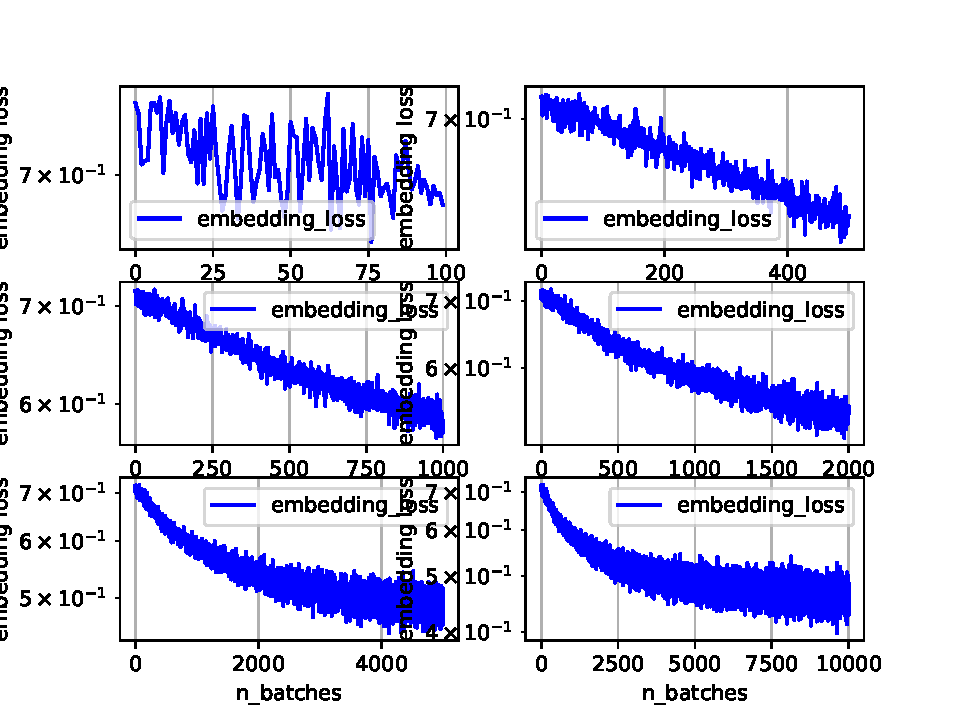
\includegraphics[width=1\textwidth]{figures/ml100k/embedding_loss_multipleplots.pdf}  
\end{center}
\caption{ml100k embedding loss with fixed alpha = 1.0}
\label{fig:ProperCover}
\end{figure}

\begin{figure}[t!]
\begin{center}
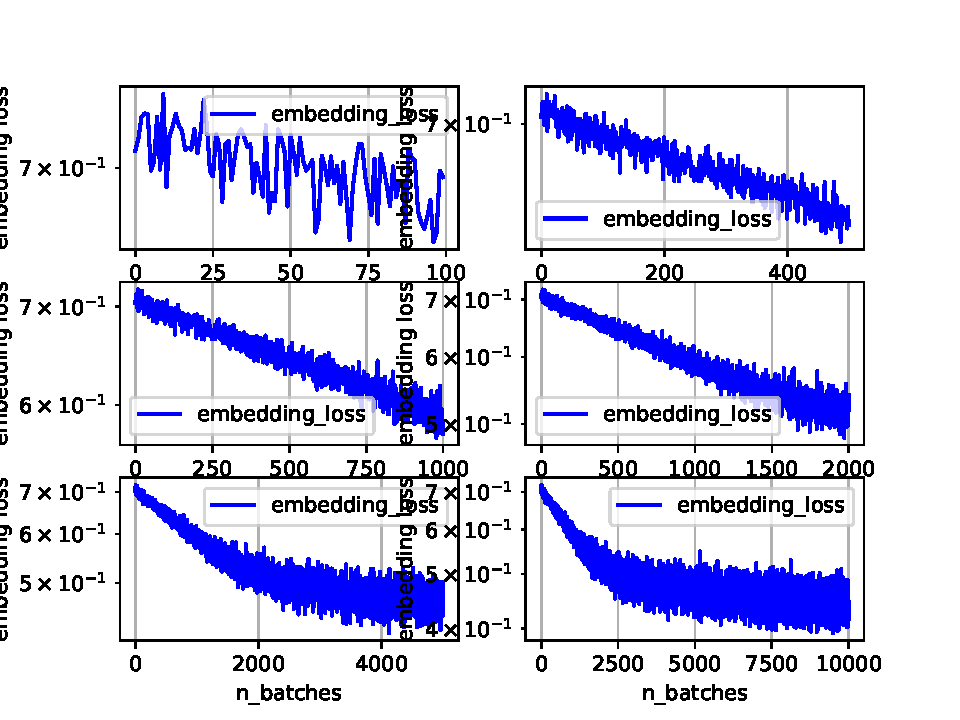
\includegraphics[width=1\textwidth]{figures/ml100k/embedding_loss_inc_alpha.pdf}  
\end{center}
\caption{ml100k embedding loss with increasing alpha. embedding loss does not seem to have converged}
\label{fig:ProperCover}
\end{figure}

\begin{figure}[t!]
\begin{center}
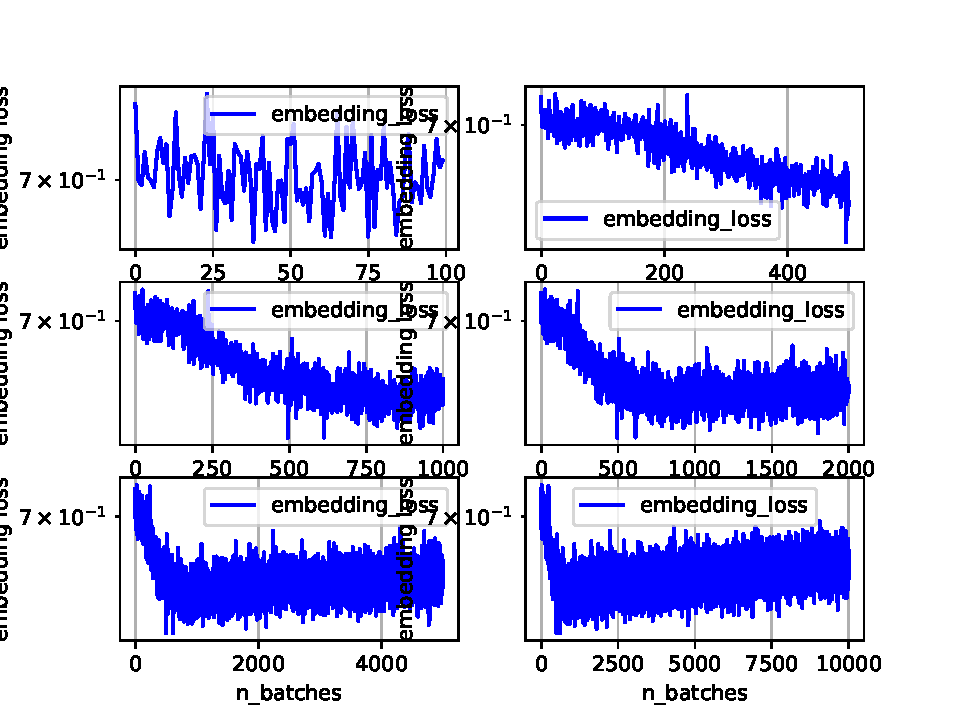
\includegraphics[width=1\textwidth]{figures/ml100k/embedding_loss_dec_alpha.pdf}  
\end{center}
\caption{ml100k embedding loss with decreasing alpha.}
\label{fig:ProperCover}
\end{figure}

\begin{figure}[t!]
\begin{center}
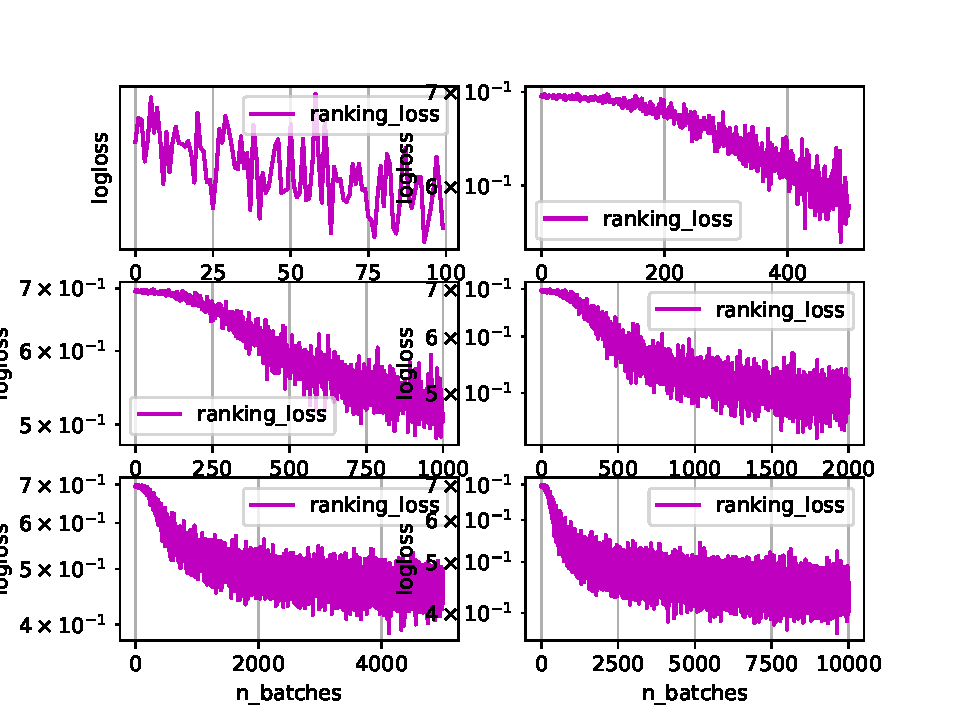
\includegraphics[width=1\textwidth]{figures/ml100k/ranking_loss_multipleplots.pdf}  
\end{center}
\caption{ml100k ranking loss with fixed alpha = 1.0}
\label{fig:ProperCover}
\end{figure}

\begin{figure}[t!]
\begin{center}
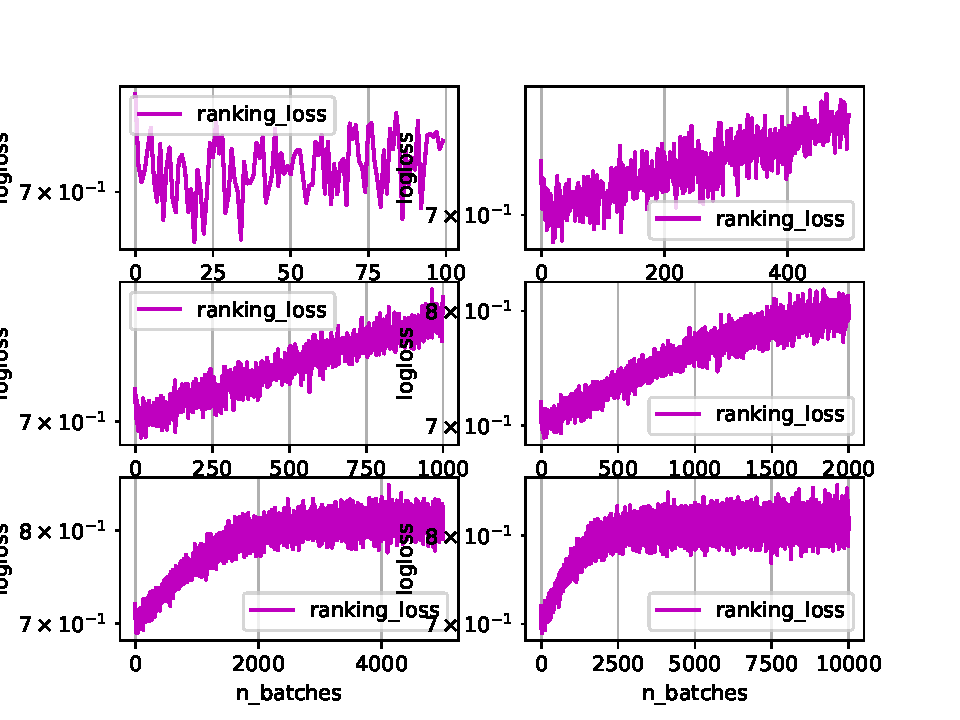
\includegraphics[width=1\textwidth]{figures/ml100k/ranking_loss_inc_alpha.pdf}  
\end{center}
\caption{ml100k ranking loss with increasing alpha. ranking loss does not seem to have converged}
\label{fig:ProperCover}
\end{figure}

\begin{figure}[t!]
\begin{center}
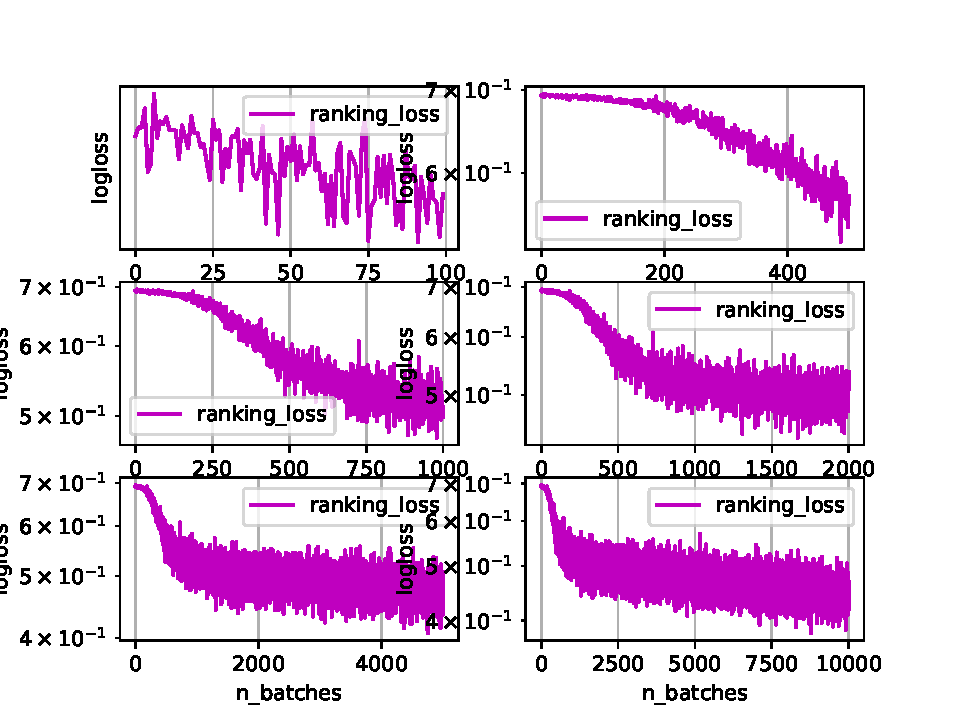
\includegraphics[width=1\textwidth]{figures/ml100k/ranking_loss_dec_alpha.pdf}  
\end{center}
\caption{ml100k ranking loss with decreasing alpha.}
\label{fig:ProperCover}
\end{figure}

\begin{figure}[t!]
\begin{center}
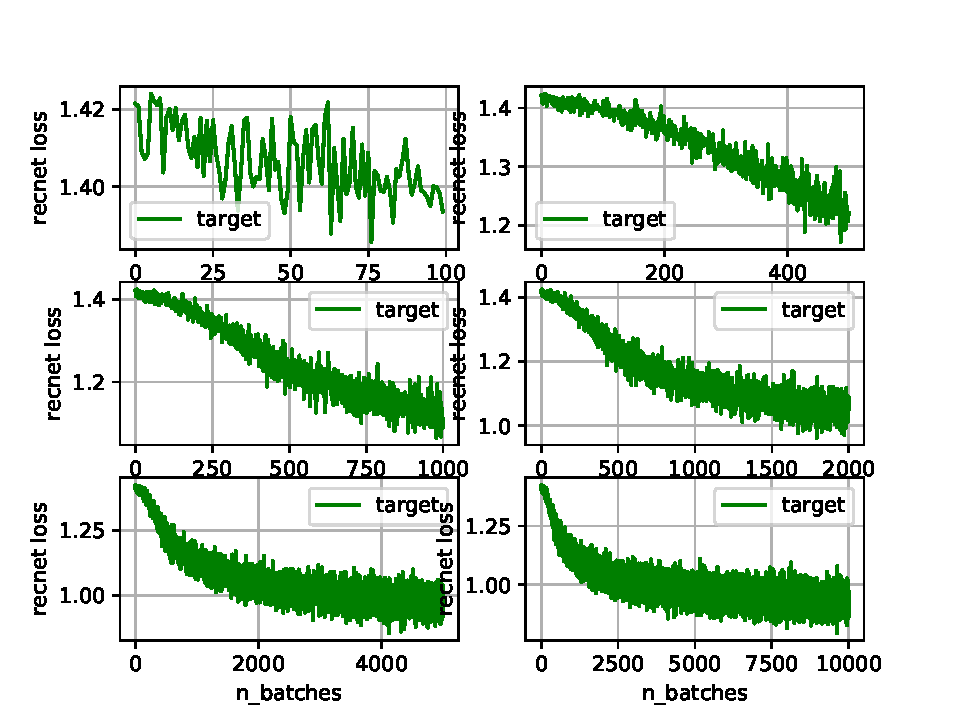
\includegraphics[width=1\textwidth]{figures/ml100k/target_loss_multipleplots.pdf}  
\end{center}
\caption{ml100k target loss with fixed alpha = 1.0}
\label{fig:ProperCover}
\end{figure}

\begin{figure}[t!]
\begin{center}
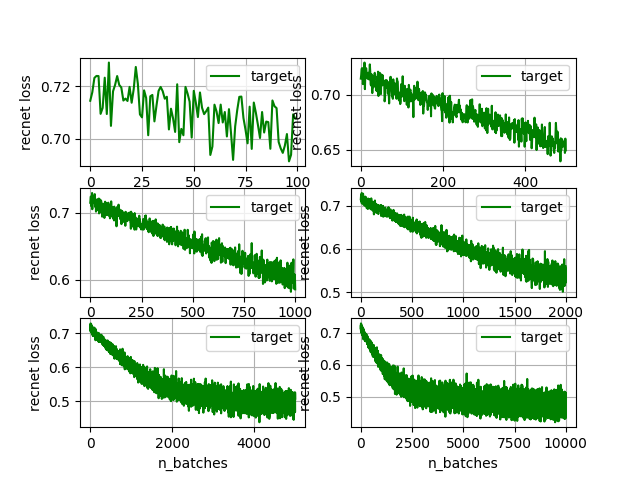
\includegraphics[width=1\textwidth]{figures/ml100k/target_loss_inc_alpha}  
\end{center}
\caption{ml100k target loss with increasing alpha. target loss does not seem to have converged}
\label{fig:ProperCover}
\end{figure}

\begin{figure}[t!]
\begin{center}
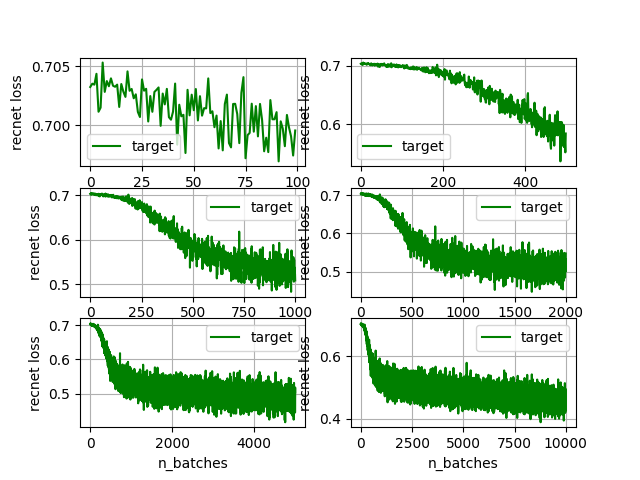
\includegraphics[width=1\textwidth]{figures/ml100k/target_loss_dec_alpha}  
\end{center}
\caption{ml100k target loss with decreasing alpha.}
\label{fig:ProperCover}
\end{figure}

\begin{table}[]
\centering
\caption{Results obtained on ML-100K. Settings with fixed $\alpha$, increasing $\alpha$ and decreasing $\alpha$}
\label{my-label}
\begin{tabular}{|c|c|c|c|}
\hline
                              & MAP@1 & MAP@5 & MAP@10 \\ \hline
$\alpha$ = 1.0, $\beta$ = 0.1 & 0.888 & 0.865 & 0.842  \\ \hline
Increase $\alpha$             &   0.819    &0.804       &   0.775     \\ \hline
Decrease $\alpha$             &   0.8375    &0.822       & 0.794       \\ \hline
\end{tabular}
\end{table}





\begin{table}[!htpb]
\centering
\caption{Best parameters for {\RecNet}$_p$, {\RecNet}$_c$ and {\RecNet}$_{c,p}$ when prediction is done on all offers; $k$ denotes the dimension of embeddings, $\lambda$ the regularization parameter. We also report the number of hidden units per layer.}
\label{tab:param}
\resizebox{\textwidth}{!}{\begin{tabular}{|c|ccc|ccc|ccc|ccc|}
\hline
                 & \multicolumn{3}{c|}{\ML-100K} & \multicolumn{3}{c|}{\ML-1M} & \multicolumn{3}{c|}{\NetF}& \multicolumn{3}{c|}{\kasandr}\\ \hline
                 &  {\RecNet}$_c$  & {\RecNet}$_p$&{\RecNet}$_{c,p}$ &{\RecNet}$_c$   &{\RecNet}$_p$ &{\RecNet}$_{c,p}$ &{\RecNet}$_c$   &{\RecNet}$_p$ &{\RecNet}$_{c,p}$&{\RecNet}$_c$   &{\RecNet}$_p$ &{\RecNet}$_{c,p}$  \\ \hline
$k$            &$15$&$5$&$8$&$8$&$1$&$1$&$14$&$2$&$4$ &18&1&18    \\
$\lambda$      &$0.001$&$0.001$&$0.001$&$0.005$&$0.0001$&$0.005$&$0.05$&$0.05$&$0.05$&0.001&0.01&0.01   \\ 
\# units &$32$&$16$&$16$&$64$&$32$&$32$&$64$&$16$& $32$ &64&64&32      \\ \hline
%\multicolumn{1}{|c|}{\# hidden layers}      &$1$&$1$&$1$&$1$&$1$&$1$&$1$&$1$&$1$     \\ \hline
%\multicolumn{1}{|c|}{$\eta$}          &$1e-3$&$1e-3$&$1e-3$&$1e-3$&$1e-3$&$1e-3$&$1e-3$&$1e-3$&$1e-3$    \\ \hline
\end{tabular}
}
\end{table}


\end{document}
